\documentclass{solutionclass} % I wrote the design using a4paper, 11pt, twoside, but feel free to change in solutionclass.cls file (line 4)

\pagestyle{plain}

\lstdefinestyle{mystyle}{
	backgroundcolor=\color{backcolour},
	commentstyle=\color{codegreen},
	keywordstyle=\color{magenta},
	numberstyle=\tiny\color{codegray},
	stringstyle=\color{codepurple},
	basicstyle=\ttfamily\normalsize,
	breakatwhitespace=false,
	breaklines=true,
	captionpos=b,
	keepspaces=true,
	numbers=left,
	numbersep=5pt,
	showspaces=false,
	showstringspaces=false,
	showtabs=false,
	tabsize=2
}

\lstset{ %
	language=Python,       % the language of the code
	basicstyle=\footnotesize,       % the size of the fonts that are used for the code
	numbers=left,                   % where to put the line-numbers
	numberstyle=\tiny\color{gray},  % the style that is used for the line-numbers
	stepnumber=1,                   % the step between two line-numbers. If it's 1, each line
	% will be numbered
	numbersep=5pt,                  % how far the line-numbers are from the code
	backgroundcolor=\color{white},  % choose the background color. You must add \usepackage{color}
	showspaces=false,               % show spaces adding particular underscores
	showstringspaces=false,         % underline spaces within strings
	showtabs=false,                 % show tabs within strings adding particular underscores
	frame=single,                   % adds a frame around the code
	rulecolor=\color{black},        % if not set, the frame-color may be changed on line-breaks within not-black text (e.g. commens (green here))
	tabsize=4,                      % sets default tabsize to 2 spaces
	breaklines=true,                % sets automatic line breaking
	breakatwhitespace=false,        % sets if automatic breaks should only happen at whitespace
	% also try caption instead of title
	keywordstyle=\color{blue}, 
    emph=[1]{for,if, end,break},emphstyle=[1]\color{red},         % keyword style
	commentstyle=\color{dkgreen},       % comment style
	stringstyle=\color{mauve},         % string literal style
	escapeinside={\%*}{*)},            % if you want to add a comment within your code
	morekeywords={*,...}               % if you want to add more keywords to the set
}

\hypersetup{
	colorlinks   = true, %Colours links instead of ugly boxes
	urlcolor     = blue, %Colour for external hyperlinks
	linkcolor    = blue, %Colour of internal links
	citecolor   = red %Colour of citations
}

\definecolor{codegreen}{rgb}{0,0.6,0}
\definecolor{codegray}{rgb}{0.5,0.5,0.5}
\definecolor{codepurple}{rgb}{0.58,0,0.82}
\definecolor{backcolour}{rgb}{0.95,0.95,0.92}
\definecolor{mGreen}{rgb}{0,0.6,0}
\definecolor{mGray}{rgb}{0.5,0.5,0.5}
\definecolor{mPurple}{rgb}{0.58,0,0.82}
\definecolor{backgroundColour}{rgb}{0.95,0.95,0.92}

\NewDocumentCommand{\codeword}{v}{
	\texttt{\textcolor{blue}{#1}}
}

\definecolor{dkgreen}{rgb}{0,0.6,0}
\definecolor{gray}{rgb}{0.5,0.5,0.5}
\definecolor{mauve}{rgb}{0.58,0,0.82}

\def\m#1{\boldsymbol{#1}}
\def\co#1{\texttt{#1}}


\begin{document}

\pretitle
{HomeWork 2} % ⟸ Write your main Title here
{Ilia Hashemi Rad}
{99102456}
{AmirMohammad Fakhimi}
{99170531}
{AmirMahdi Namjoo}
{97107212}

% Change your homework number here
\def\homeworkNumber{2}

\makeatletter
    \startcontents[sections]
    \phantomsection
\makeatother
    \def\Solu{Explanations}

\section{Introduction}

\begin{solution}
In this project we have implemented a classification problem on sentiment analysis both on a document and text level on Taaghche comments dataset. Taaghche is a Iranian online ebook marketplace that features user comments for each book. Based on a dataset of scores and comments of users and other users' likes on the comments, we implemented a classifier for setniment analysis of the text. We use both base models like LSTM or SVM and also Transfomer-based models.

In addition to this, we also wrote a crawler Taaghche website to crawl all the book pages and get the book information like name and author names so that we can have a list of NER for them.

\end{solution}


\section{Crawlers}

\begin{solution}
In the first part, we implemented a crawler on Taaghche website to get all the books info. The crawler download the pages of all books on the website by iterating on the "id" in the url and save the result as HTML. We then feed the results into a extractor module written using BeautifulSoup to extract the main parts of a book info including name, publication, author, translator, etc. and save them into csv files for further use.
\end{solution}

\subsection*{\co{crawler.py}}
\begin{lstlisting}[language=Python]
base_url = "https://taaghche.com/book/"
def save_page(book_id, thread_exceptions):
	url = f"{base_url}{book_id}/"
	try:
		response = requests.get(url)
		
		if response.status_code == 404:
			print(book_id," : 404")
			return
		
		with open(os.path.join(output_dir, f"{book_id}.html"), 'w', encoding='utf-8') as f:
			print(f'Saving book with id: {book_id}')
			f.write(response.text)
	except Exception as e:
		print(e)
		thread_exceptions.append(book_id)
\begin{solution}
This is the main part of crawler that sends request to Taagche to get the book pages and save them into files. We also used python threading features to make the whole process faster.


\end{solution}

\subsection*{\co{extactor.py}}
\begin{lstlisting}[language=Python]
    def extract_data_from_html(file_path):
    with open(file_path, 'r', encoding='utf-8') as file:
        soup = BeautifulSoup(file, 'html.parser')
        script_tag = soup.find('script', type='application/ld+json')
        if script_tag:
            try:
                json_data = json.loads(script_tag.string)
                book_name = json_data.get('name', '')
                authors = ' $ '.join([author['name'] for author in json_data.get('author', [])])
                translators = ' $ '.join(
                    [translator['name'] for translator in json_data.get('workExample', {}).get('translator', [])])
                publisher = json_data.get('workExample', {}).get('publisher', {}).get('name', '')
                data.append({
                    'name': book_name,
                    'author': authors,
                    'translator': translators,
                    'publisher': publisher
                })
            except json.JSONDecodeError:
                pass

    for x in os.listdir(input_dir):
    file_name = x
    file_path = os.path.join(input_dir, file_name)
    if os.path.isfile(file_path) and file_path.endswith('.html'):
        extract_data_from_html(file_path)
    if len(data) >= 10000:
        df = pd.DataFrame(data)
        output_file = os.path.join(output_dir, f'books_data_part_{part_number}.csv')
        df.to_csv(output_file, index=False, encoding='utf-8')
        data = []
        part_number += 1
        print("index put into files: ", file_name)

if data:
    df = pd.DataFrame(data)
    output_file = os.path.join(output_dir, f'books_data_part_{part_number}.csv')
    df.to_csv(output_file, index=False, encoding='utf-8')
    data = []
    part_number += 1
    print("index put into files: ", file_name)
    data = []
\end{lstlisting}

\begin{solution}
The main part of extracor.py is \co{extract\_data\_from\_html} function. This function uses BS4 to find the JSON section that includes book data in the HTML and save data json data into a python dictionary. This data is then fed into a Pandas Dataframe and we save it into a csv file.


\end{solution}

\section{Document Classifier}

The base model is in \co{DocClassifier\_Base.ipynb}. We investigate each segment in the following sections.

\subsection*{Loading and Preparing Data}


\begin{lstlisting}[language=Python]
# Import the pandas library for data manipulation
import pandas as pd

# Load the CSV file into a pandas DataFrame
# The file 'taghche.csv' is located in the 'datasets/' directory
data = pd.read_csv('datasets/taghche.csv')

# Remove any duplicate rows in the DataFrame
data = data.drop_duplicates()

# Drop rows where the 'comment' or 'rate' columns have missing values (NaN)
data.dropna(subset=['comment', 'rate'], inplace=True)

# Print the first 5 rows of the cleaned DataFrame
print(data.head())


def label_sentiment(rate, positive_threshold, neutral_threshold):
"""
Labels sentiment based on rating thresholds.

Args:
- rate (int or float): The numerical rating to evaluate.
- positive_threshold (int or float): The minimum rating value that qualifies as 'positive'.
- neutral_threshold (int or float): The minimum rating value that qualifies as 'neutral'; ratings below this are considered 'negative'.

Returns:
- str: The sentiment label ('positive', 'neutral', or 'negative') based on the rating.
"""
# Check if the rating is greater than or equal to the positive threshold
if rate >= positive_threshold:
return 'positive'
# If the rating is not 'positive', check if it is greater than or equal to the neutral threshold
elif rate >= neutral_threshold:
return 'neutral'
# If the rating is neither 'positive' nor 'neutral', label the sentiment as 'negative'
else:
return 'negative'
\end{lstlisting}

\begin{solution}
At first, we load data using Pandas Library. We then define a fucntion to label the sentiment of each comment based on its rating and threshold. note that we have two thresholds, one for positive, and one for neutral comments. everything below neutral is considered negative.
\end{solution}



\subsection*{Balancing Data}


\begin{lstlisting}[language=Python]
	# Function to prepare data and labels based on given thresholds
def prepare_data(positive_threshold, neutral_threshold):
    """
    Prepares the data and labels based on given thresholds for sentiment classification.

    Args:
    - positive_threshold (int or float): The minimum rating value that qualifies as 'positive'.
    - neutral_threshold (int or float): The minimum rating value that qualifies as 'neutral'; ratings below this are considered 'negative'.

    Returns:
    - tuple: A tuple containing:
        - pandas.Series: The comments from the balanced dataset.
        - pandas.Series: The corresponding sentiment labels from the balanced dataset.
    """
    # Create a copy of the original data to avoid modifying it
    labeled_data = data.copy()
    
    # Apply the label_sentiment function to the 'rate' column to create a new 'sentiment' column
    labeled_data['sentiment'] = labeled_data['rate'].apply(lambda x: label_sentiment(x, positive_threshold, neutral_threshold))
    
    # Combine the 'comment' and 'sentiment' columns into a single DataFrame
    df = pd.concat([labeled_data['comment'], labeled_data['sentiment']], axis=1)

    # Separate the DataFrame into three classes based on sentiment
    positive = df[df['sentiment'] == 'positive']
    neutral = df[df['sentiment'] == 'neutral']
    negative = df[df['sentiment'] == 'negative']

    # Determine the size of the smallest class to balance the dataset
    min_class_size = min(len(positive), len(neutral), len(negative))

    # Downsample each class to the size of the smallest class to ensure balance
    positive_downsampled = resample(positive, replace=False, n_samples=min_class_size, random_state=42)
    neutral_downsampled = resample(neutral, replace=False, n_samples=min_class_size, random_state=42)
    negative_downsampled = resample(negative, replace=False, n_samples=min_class_size, random_state=42)

    # Combine the downsampled classes into a single DataFrame
    df_balanced = pd.concat([positive_downsampled, neutral_downsampled, negative_downsampled])

    # Shuffle the balanced DataFrame to mix the rows
    df_balanced = df_balanced.sample(frac=1, random_state=42).reset_index(drop=True)
    
    # Return the 'comment' and 'sentiment' columns as separate pandas Series
    return df_balanced['comment'], df_balanced['sentiment']
\end{lstlisting}

\begin{solution}
\begin{itemize}
	\item The function starts by creating a copy of the original dataset to avoid modifying it:
	\begin{lstlisting}[language=Python]
		labeled_data = data.copy()
	\end{lstlisting}
	
	\item It applies the \texttt{label\_sentiment} function to the \texttt{rate} column to create a new \texttt{sentiment} column:
	\begin{lstlisting}[language=Python]
		labeled_data['sentiment'] = labeled_data['rate'].apply(lambda x: label_sentiment(x, positive_threshold, neutral_threshold))
	\end{lstlisting}
	
	\item The function then combines the \texttt{comment} and \texttt{sentiment} columns into a single DataFrame:
	\begin{lstlisting}[language=Python]
		df = pd.concat([labeled_data['comment'], labeled_data['sentiment']], axis=1)
	\end{lstlisting}
	
	\item It separates the DataFrame into three classes based on sentiment:
	\begin{lstlisting}[language=Python]
		positive = df[df['sentiment'] == 'positive']
		neutral = df[df['sentiment'] == 'neutral']
		negative = df[df['sentiment'] == 'negative']
	\end{lstlisting}
	
	\item The function determines the size of the smallest class to balance the dataset:
	\begin{lstlisting}[language=Python]
		min_class_size = min(len(positive), len(neutral), len(negative))
	\end{lstlisting}
	
	\item It down-samples each class to the size of the smallest class to ensure balance:
	\begin{lstlisting}[language=Python]
		positive_downsampled = resample(positive, replace=False, n_samples=min_class_size, random_state=42)
		neutral_downsampled = resample(neutral, replace=False, n_samples=min_class_size, random_state=42)
		negative_downsampled = resample(negative, replace=False, n_samples=min_class_size, random_state=42)
	\end{lstlisting}
	
	\item The function combines the down-sampled classes into a single DataFrame:
	\begin{lstlisting}[language=Python]
		df_balanced = pd.concat([positive_downsampled, neutral_downsampled, negative_downsampled])
	\end{lstlisting}
	
	\item It shuffles the balanced DataFrame to mix the rows:
	\begin{lstlisting}[language=Python]
		df_balanced = df_balanced.sample(frac=1, random_state=42).reset_index(drop=True)
	\end{lstlisting}
	
	\item Finally, the function returns the \texttt{comment} and \texttt{sentiment} columns as separate pandas Series:
	\begin{lstlisting}[language=Python]
		return df_balanced['comment'], df_balanced['sentiment']
	\end{lstlisting}
\end{itemize}
\end{solution}




\subsection*{Preprocess}


\begin{lstlisting}[language=Python]
	# Function to preprocess and normalize the text
def preprocess(text):
    """
    Preprocesses and normalizes text data by removing special characters,
    non-Persian characters, digits, and multiple spaces.

    Args:
    - text (str): Input text to be processed.

    Returns:
    - str: Processed text with normalized format.
    """
    # Replace one or more newline characters with a single newline
    pattern = re.compile(r"\n+")
    text = pattern.sub("\n", text)
    
    # Replace '\n' and '\n' with a single space
    text = re.sub(r'\\n|\n', ' ', text)
    
    # Remove non-Persian characters and digits
    text = re.sub(r'[^آ-ی\s]', ' ', text)
    
    # Replace one or more spaces with a single space
    pattern = re.compile(r" +")
    text = pattern.sub(" ", text)
    
    return text

# Apply the preprocess function to the 'comment' column in the DataFrame data
data['comment'] = data['comment'].apply(preprocess)
# Remove any duplicate rows in the DataFrame
data = data.drop_duplicates()

# Drop rows where the 'comment' or 'rate' columns have missing values (NaN)
data.dropna(subset=['comment', 'rate'], inplace=True)
\end{lstlisting}

\begin{solution}
	\begin{itemize}
        \item The function starts by replacing one or more newline characters with a single newline:
        \begin{lstlisting}[language=Python]
        pattern = re.compile(r"\n+")
        text = pattern.sub("\n", text)
        \end{lstlisting}
    
        \item Next, it replaces occurrences of the newline character (\verb*|\n|) and escaped newline (\verb*|\\n|) with a single space:
        \begin{lstlisting}[language=Python]
        text = re.sub(r'\\n|\n', ' ', text)
        \end{lstlisting}
    
        \item The function then removes all non-Persian characters and digits. This is done using a regular expression that matches any character not in the Persian alphabet (آ-ی) or whitespace:
        \begin{lstlisting}[language=Python]
        text = re.sub(r'[^آ-ی\s]', ' ', text)
        \end{lstlisting}
    
        \item Finally, it replaces one or more spaces with a single space to normalize the spacing in the text:
        \begin{lstlisting}[language=Python]
        pattern = re.compile(r" +")
        text = pattern.sub(" ", text)
        \end{lstlisting}
    
        \item The processed text is then returned by the function.
    \end{itemize}
    
    The following lines apply the \texttt{preprocess} function to the \texttt{comment} column of the DataFrame \texttt{data}:
    
    \begin{lstlisting}[language=Python]
    # Apply the preprocess function to the 'comment' column in the DataFrame data
    data['comment'] = data['comment'].apply(preprocess)
    
    # Remove any duplicate rows in the DataFrame
    data = data.drop_duplicates()
    
    # Drop rows where the 'comment' or 'rate' columns have missing values (NaN)
    data.dropna(subset=['comment', 'rate'], inplace=True)
    \end{lstlisting}
    
    \begin{itemize}
        \item The \texttt{preprocess} function is applied to each entry in the \texttt{comment} column to clean and normalize the text.
        \item After preprocessing, any duplicate rows in the DataFrame are removed using:
        \begin{lstlisting}[language=Python]
        data = data.drop_duplicates()
        \end{lstlisting}
        \item Finally, rows where the \texttt{comment} or \texttt{rate} columns have missing values (NaN) are dropped:
        \begin{lstlisting}[language=Python]
        data.dropna(subset=['comment', 'rate'], inplace=True)
        \end{lstlisting}
    \end{itemize}
    
\end{solution}




\subsection*{TF IDF - Logistic Regression}

Next we implement a TF-IDF vectorizer and use logistic regresson for the task.



\begin{lstlisting}[language=Python]
	# Create a pipeline with TF-IDF and logistic regression
logReg_PL = Pipeline([
    ("tfidf", TfidfVectorizer()),
    ("logreg", LogisticRegression(max_iter=500, solver='newton-cg'))
])

# Define the parameter grid for GridSearchCV
param_grid = {
    'tfidf__ngram_range': [(1, 1), (1, 2), (1, 3)],
    'tfidf__max_features': [5000, 10000],
    'logreg__C': [0.01, 0.1, 1, 10]
}

# Custom GridSearchCV implementation to iterate over parameter grid
best_score = 0
best_params = None

# Thresholds to evaluate
rate_thresholds = [(1, 2), (1, 3), (1, 4), (2, 3), (2, 4), (3, 4)]

# Iterate over each pair of thresholds and perform GridSearchCV
for neutral_threshold, positive_threshold in tqdm(rate_thresholds):
    # Prepare the data using the specified thresholds
    X_prepared, y_prepared = prepare_data(positive_threshold, neutral_threshold)
    
    # Split the data into training and testing sets
    X_train, X_test, y_train, y_test = train_test_split(X_prepared, y_prepared, test_size=0.1, random_state=42)
    
    # Initialize GridSearchCV with the pipeline and parameter grid
    grid_search = GridSearchCV(logReg_PL, param_grid, cv=5, scoring='accuracy')
    
    # Fit GridSearchCV on the training data
    grid_search.fit(X_train, y_train)
    
    # Get the best score and parameters from GridSearchCV
    score = grid_search.best_score_
    
    # Update the best score and best parameters if the current score is better
    if score > best_score:
        best_score = score
        best_params = grid_search.best_params_
        best_params['positive_threshold'] = positive_threshold
        best_params['neutral_threshold'] = neutral_threshold

# Print the best parameters found by GridSearchCV
print("Best parameters for TF-IDF model are:", best_params)

# Prepare the data using the best parameters found from GridSearchCV
X_prepared, y_prepared = prepare_data(best_params['positive_threshold'], best_params['neutral_threshold'])

# Split the prepared data into training and testing sets
X_train, X_test, y_train, y_test = train_test_split(X_prepared, y_prepared, test_size=0.1, random_state=42)

# Create a pipeline for the best Logistic Regression model with the best parameters
best_logReg_model = Pipeline([
    ("tfidf", TfidfVectorizer(ngram_range=best_params['tfidf__ngram_range'], max_features=best_params['tfidf__max_features'])),
    ("logreg", LogisticRegression(C=best_params['logreg__C'], max_iter=500, solver='newton-cg'))
])

# Fit the best Logistic Regression model on the training data
best_logReg_model.fit(X_train, y_train)

# Predict the labels on the test set using the best model
y_test_pred = best_logReg_model.predict(X_test)

# Calculate the accuracy score of the best model on the test set
test_accuracy = accuracy_score(y_test, y_test_pred)

# Print the test accuracy score of the best Logistic Regression model
print("Test accuracy of Logistic Regression model:", test_accuracy)
\end{lstlisting}

\begin{solution}
	\begin{lstlisting}[language=Python]
        logReg_PL = Pipeline([
            ("tfidf", TfidfVectorizer()),
            ("logreg", LogisticRegression(max_iter=500, solver='newton-cg'))
        ])
        \end{lstlisting}
        
        \begin{itemize}
            \item The pipeline \texttt{logReg\_PL} is created with two steps:
            \begin{enumerate}
                \item \texttt{TfidfVectorizer()}: Converts text data into TF-IDF features.
                \item \texttt{LogisticRegression()}: Applies logistic regression for classification, with a maximum of 500 iterations and the 'newton-cg' solver.
            \end{enumerate}
        \end{itemize}
        
        \begin{lstlisting}[language=Python]
        # Define the parameter grid for GridSearchCV
        param_grid = {
            'tfidf__ngram_range': [(1, 1), (1, 2), (1, 3)],
            'tfidf__max_features': [5000, 10000],
            'logreg__C': [0.01, 0.1, 1, 10]
        }
        \end{lstlisting}
        
        \begin{itemize}
            \item The \texttt{param\_grid} defines the hyperparameters for GridSearchCV to search over:
            \begin{itemize}
                \item \texttt{tfidf\_\_ngram\_range}: N-gram ranges (unigrams, bigrams, trigrams).
                \item \texttt{tfidf\_\_max\_features}: Maximum number of features (5000 or 10000).
                \item \texttt{logreg\_\_C}: Inverse of regularization strength (0.01, 0.1, 1, 10).
            \end{itemize}
        \end{itemize}
        
        \begin{lstlisting}[language=Python]
        # Custom GridSearchCV implementation to iterate over parameter grid
        best_score = 0
        best_params = None
        
        # Thresholds to evaluate
        rate_thresholds = [(1, 2), (1, 3), (1, 4), (2, 3), (2, 4), (3, 4)]
        \end{lstlisting}
        
        \begin{itemize}
            \item \texttt{best\_score} and \texttt{best\_params} are initialized to store the best score and corresponding parameters.
            \item \texttt{rate\_thresholds} contains pairs of thresholds to evaluate for neutral and positive sentiment classification.
        \end{itemize}
        
        \begin{lstlisting}[language=Python]
        # Iterate over each pair of thresholds and perform GridSearchCV
        for neutral_threshold, positive_threshold in tqdm(rate_thresholds):
            # Prepare the data using the specified thresholds
            X_prepared, y_prepared = prepare_data(positive_threshold, neutral_threshold)
            
            # Split the data into training and testing sets
            X_train, X_test, y_train, y_test = train_test_split(X_prepared, y_prepared, test_size=0.1, random_state=42)
            
            # Initialize GridSearchCV with the pipeline and parameter grid
            grid_search = GridSearchCV(logReg_PL, param_grid, cv=5, scoring='accuracy')
            
            # Fit GridSearchCV on the training data
            grid_search.fit(X_train, y_train)
            
            # Get the best score and parameters from GridSearchCV
            score = grid_search.best_score_
            
            # Update the best score and best parameters if the current score is better
            if score > best_score:
                best_score = score
                best_params = grid_search.best_params_
                best_params['positive_threshold'] = positive_threshold
                best_params['neutral_threshold'] = neutral_threshold
        
        # Print the best parameters found by GridSearchCV
        print("Best parameters for TF-IDF model are:", best_params)
        \end{lstlisting}
        
        \begin{itemize}
            \item The code iterates over each pair of thresholds in \texttt{rate\_thresholds}.
            \item For each pair:
            \begin{enumerate}
                \item \texttt{prepare\_data} is called to prepare the dataset with the current thresholds.
                \item The data is split into training and testing sets using \texttt{train\_test\_split}.
                \item \texttt{GridSearchCV} is initialized with the pipeline and parameter grid, and fitted to the training data.
                \item The best score and parameters are retrieved from the grid search results.
                \item If the current score is better than the best score, update \texttt{best\_score} and \texttt{best\_params}.
            \end{enumerate}
        \end{itemize}
        
        \begin{lstlisting}[language=Python]
        # Prepare the data using the best parameters found from GridSearchCV
        X_prepared, y_prepared = prepare_data(best_params['positive_threshold'], best_params['neutral_threshold'])
        
        # Split the prepared data into training and testing sets
        X_train, X_test, y_train, y_test = train_test_split(X_prepared, y_prepared, test_size=0.1, random_state=42)
        
        # Create a pipeline for the best Logistic Regression model with the best parameters
        best_logReg_model = Pipeline([
            ("tfidf", TfidfVectorizer(ngram_range=best_params['tfidf__ngram_range'], max_features=best_params['tfidf__max_features'])),
            ("logreg", LogisticRegression(C=best_params['logreg__C'], max_iter=500, solver='newton-cg'))
        ])
        
        # Fit the best Logistic Regression model on the training data
        best_logReg_model.fit(X_train, y_train)
        
        # Predict the labels on the test set using the best model
        y_test_pred = best_logReg_model.predict(X_test)
        
        # Calculate the accuracy score of the best model on the test set
        test_accuracy = accuracy_score(y_test, y_test_pred)
        
        # Print the test accuracy score of the best Logistic Regression model
        print("Test accuracy of Logistic Regression model:", test_accuracy)
        \end{lstlisting}
        
        \begin{itemize}
            \item The data is prepared using the best parameters found by GridSearchCV.
            \item The prepared data is split into training and testing sets.
            \item A pipeline is created for the best logistic regression model with the best parameters.
            \item The model is fitted to the training data.
            \item Predictions are made on the test set.
            \item The accuracy of the model is calculated on the test set.
            \item The test accuracy is printed.
        \end{itemize}
        
\end{solution}




\subsection*{Evaluation Metrics}


\begin{lstlisting}[language=Python]
	def evaluate_model(y_true, y_pred, class_names):
    """
    Evaluates the performance of a classification model using various metrics and visualizations.

    Args:
    - y_true (array-like): True labels of the data.
    - y_pred (array-like): Predicted labels of the data.
    - class_names (list): List of class names in the same order as the confusion matrix.

    Returns:
    - pd.DataFrame: DataFrame containing the classification report.
    """
    # Generate and print the classification report
    report = classification_report(y_true, y_pred, target_names=class_names, output_dict=True)
    report_df = pd.DataFrame(report).transpose()
    print("Classification Report:\n", report_df)

    # Generate and display the confusion matrix as a heatmap
    cm = confusion_matrix(y_true, y_pred)
    plt.figure(figsize=(10, 7))
    sns.heatmap(cm, annot=True, fmt='d', cmap='Blues', xticklabels=class_names, yticklabels=class_names)
    plt.xlabel('Predicted')
    plt.ylabel('True')
    plt.title('Confusion Matrix')
    plt.show()

    # Calculate and print overall metrics: accuracy, precision, recall, and F1 score
    accuracy = accuracy_score(y_true, y_pred)
    precision = precision_score(y_true, y_pred, average='weighted')
    recall = recall_score(y_true, y_pred, average='weighted')
    f1 = f1_score(y_true, y_pred, average='weighted')

    metrics = {
        "Accuracy": accuracy,
        "Precision": precision,
        "Recall": recall,
        "F1 Score": f1
    }

    print("\nOverall Metrics:")
    for metric, value in metrics.items():
        print(f"{metric}: {value:.4f}")
    
    return report_df

# Evaluate the model
report_df = evaluate_model(y_test, y_test_pred, ["Negative", "Neutral", "Positive"])
\end{lstlisting}

\begin{solution}
	The \texttt{evaluate\_model} function evaluates the performance of a classification model using various metrics and visualizations.
\begin{itemize}
    \item The function takes three arguments:
    \begin{itemize}
        \item \texttt{y\_true}: The true labels of the data.
        \item \texttt{y\_pred}: The predicted labels of the data.
        \item \texttt{class\_names}: A list of class names in the same order as the confusion matrix.
    \end{itemize}
    \item The function returns a pandas DataFrame containing the classification report.
\end{itemize}

\subsection*{Classification Report}

\begin{itemize}
    \item The classification report is generated using \texttt{classification\_report} from scikit-learn and printed:
    \begin{lstlisting}[language=Python]
    report = classification_report(y_true, y_pred, target_names=class_names, output_dict=True)
    report_df = pd.DataFrame(report).transpose()
    print("Classification Report:\n", report_df)
    \end{lstlisting}
\end{itemize}

\subsection*{Confusion Matrix}

\begin{itemize}
    \item The confusion matrix is generated and displayed as a heatmap using seaborn:
    \begin{lstlisting}[language=Python]
    cm = confusion_matrix(y_true, y_pred)
    plt.figure(figsize=(10, 7))
    sns.heatmap(cm, annot=True, fmt='d', cmap='Blues', xticklabels=class_names, yticklabels=class_names)
    plt.xlabel('Predicted')
    plt.ylabel('True')
    plt.title('Confusion Matrix')
    plt.show()
    \end{lstlisting}
\end{itemize}

\subsection*{Overall Metrics}

\begin{itemize}
    \item The function calculates and prints overall metrics including accuracy, precision, recall, and F1 score:
    \begin{lstlisting}[language=Python]
    accuracy = accuracy_score(y_true, y_pred)
    precision = precision_score(y_true, y_pred, average='weighted')
    recall = recall_score(y_true, y_pred, average='weighted')
    f1 = f1_score(y_true, y_pred, average='weighted')

    metrics = {
        "Accuracy": accuracy,
        "Precision": precision,
        "Recall": recall,
        "F1 Score": f1
    }

    print("\nOverall Metrics:")
    for metric, value in metrics.items():
        print(f"{metric}: {value:.4f}")
    \end{lstlisting}
    \item These metrics are printed in a readable format.
\end{itemize}

\subsection*{Function Return}

\begin{itemize}
    \item The function returns the classification report DataFrame:
    \begin{lstlisting}[language=Python]
    return report_df
    \end{lstlisting}
\end{itemize}

\subsection*{Model Evaluation}

\begin{itemize}
    \item The \texttt{evaluate\_model} function is called to evaluate the model:
    \begin{lstlisting}[language=Python]
    report_df = evaluate_model(y_test, y_test_pred, ["Negative", "Neutral", "Positive"])
    \end{lstlisting}
\end{itemize}
\end{solution}


\subsection{Results and Interesting Notes}

For the results section, we analyzed different approaches on the data to check whether we can get a better result or not. At first, we tested it without any special technique and got an accuracy of about 0.61 on the whole data. another approach we tested is removing stopwords, but interestingly, it seems stopwords are important for our task and after removing them, or accuracy dropped.


Another approach was to use a formalizer to change the text into a fomral persian text. We used a formalizer based on T5 using models from previous semesters, but we got worse results. It is predictable though, because some informal persian slangs can greatly change the sentiment of a sentence and they lose their meaning even in a human perspective when we formalize them.

We also used another approach for fomralization; Giving the persian text to Google Translate to translate it into English and then translate it back into persian. It didn't work fine either.

One of the things we find in papers that seem good for this task, is lemmetizer. We tried to use it on our data but unfortuantely, Hazm was very slow on our 70K database in we could not use this technique for our task.

It seems or result is good enough though. As it is a multiclass classification and the best results are for ParsBERT on an extermely larger database than ours that is near 70\%, so it seems our accuracy of 61\% is good enough.



\subsection*{Loading Data}


\begin{lstlisting}[language=Python]
	Test
\end{lstlisting}

\begin{solution}
	Test
\end{solution}



\subsection*{Loading Data}


\begin{lstlisting}[language=Python]
	Test
\end{lstlisting}

\begin{solution}
	Test
\end{solution}

\begin{center}
  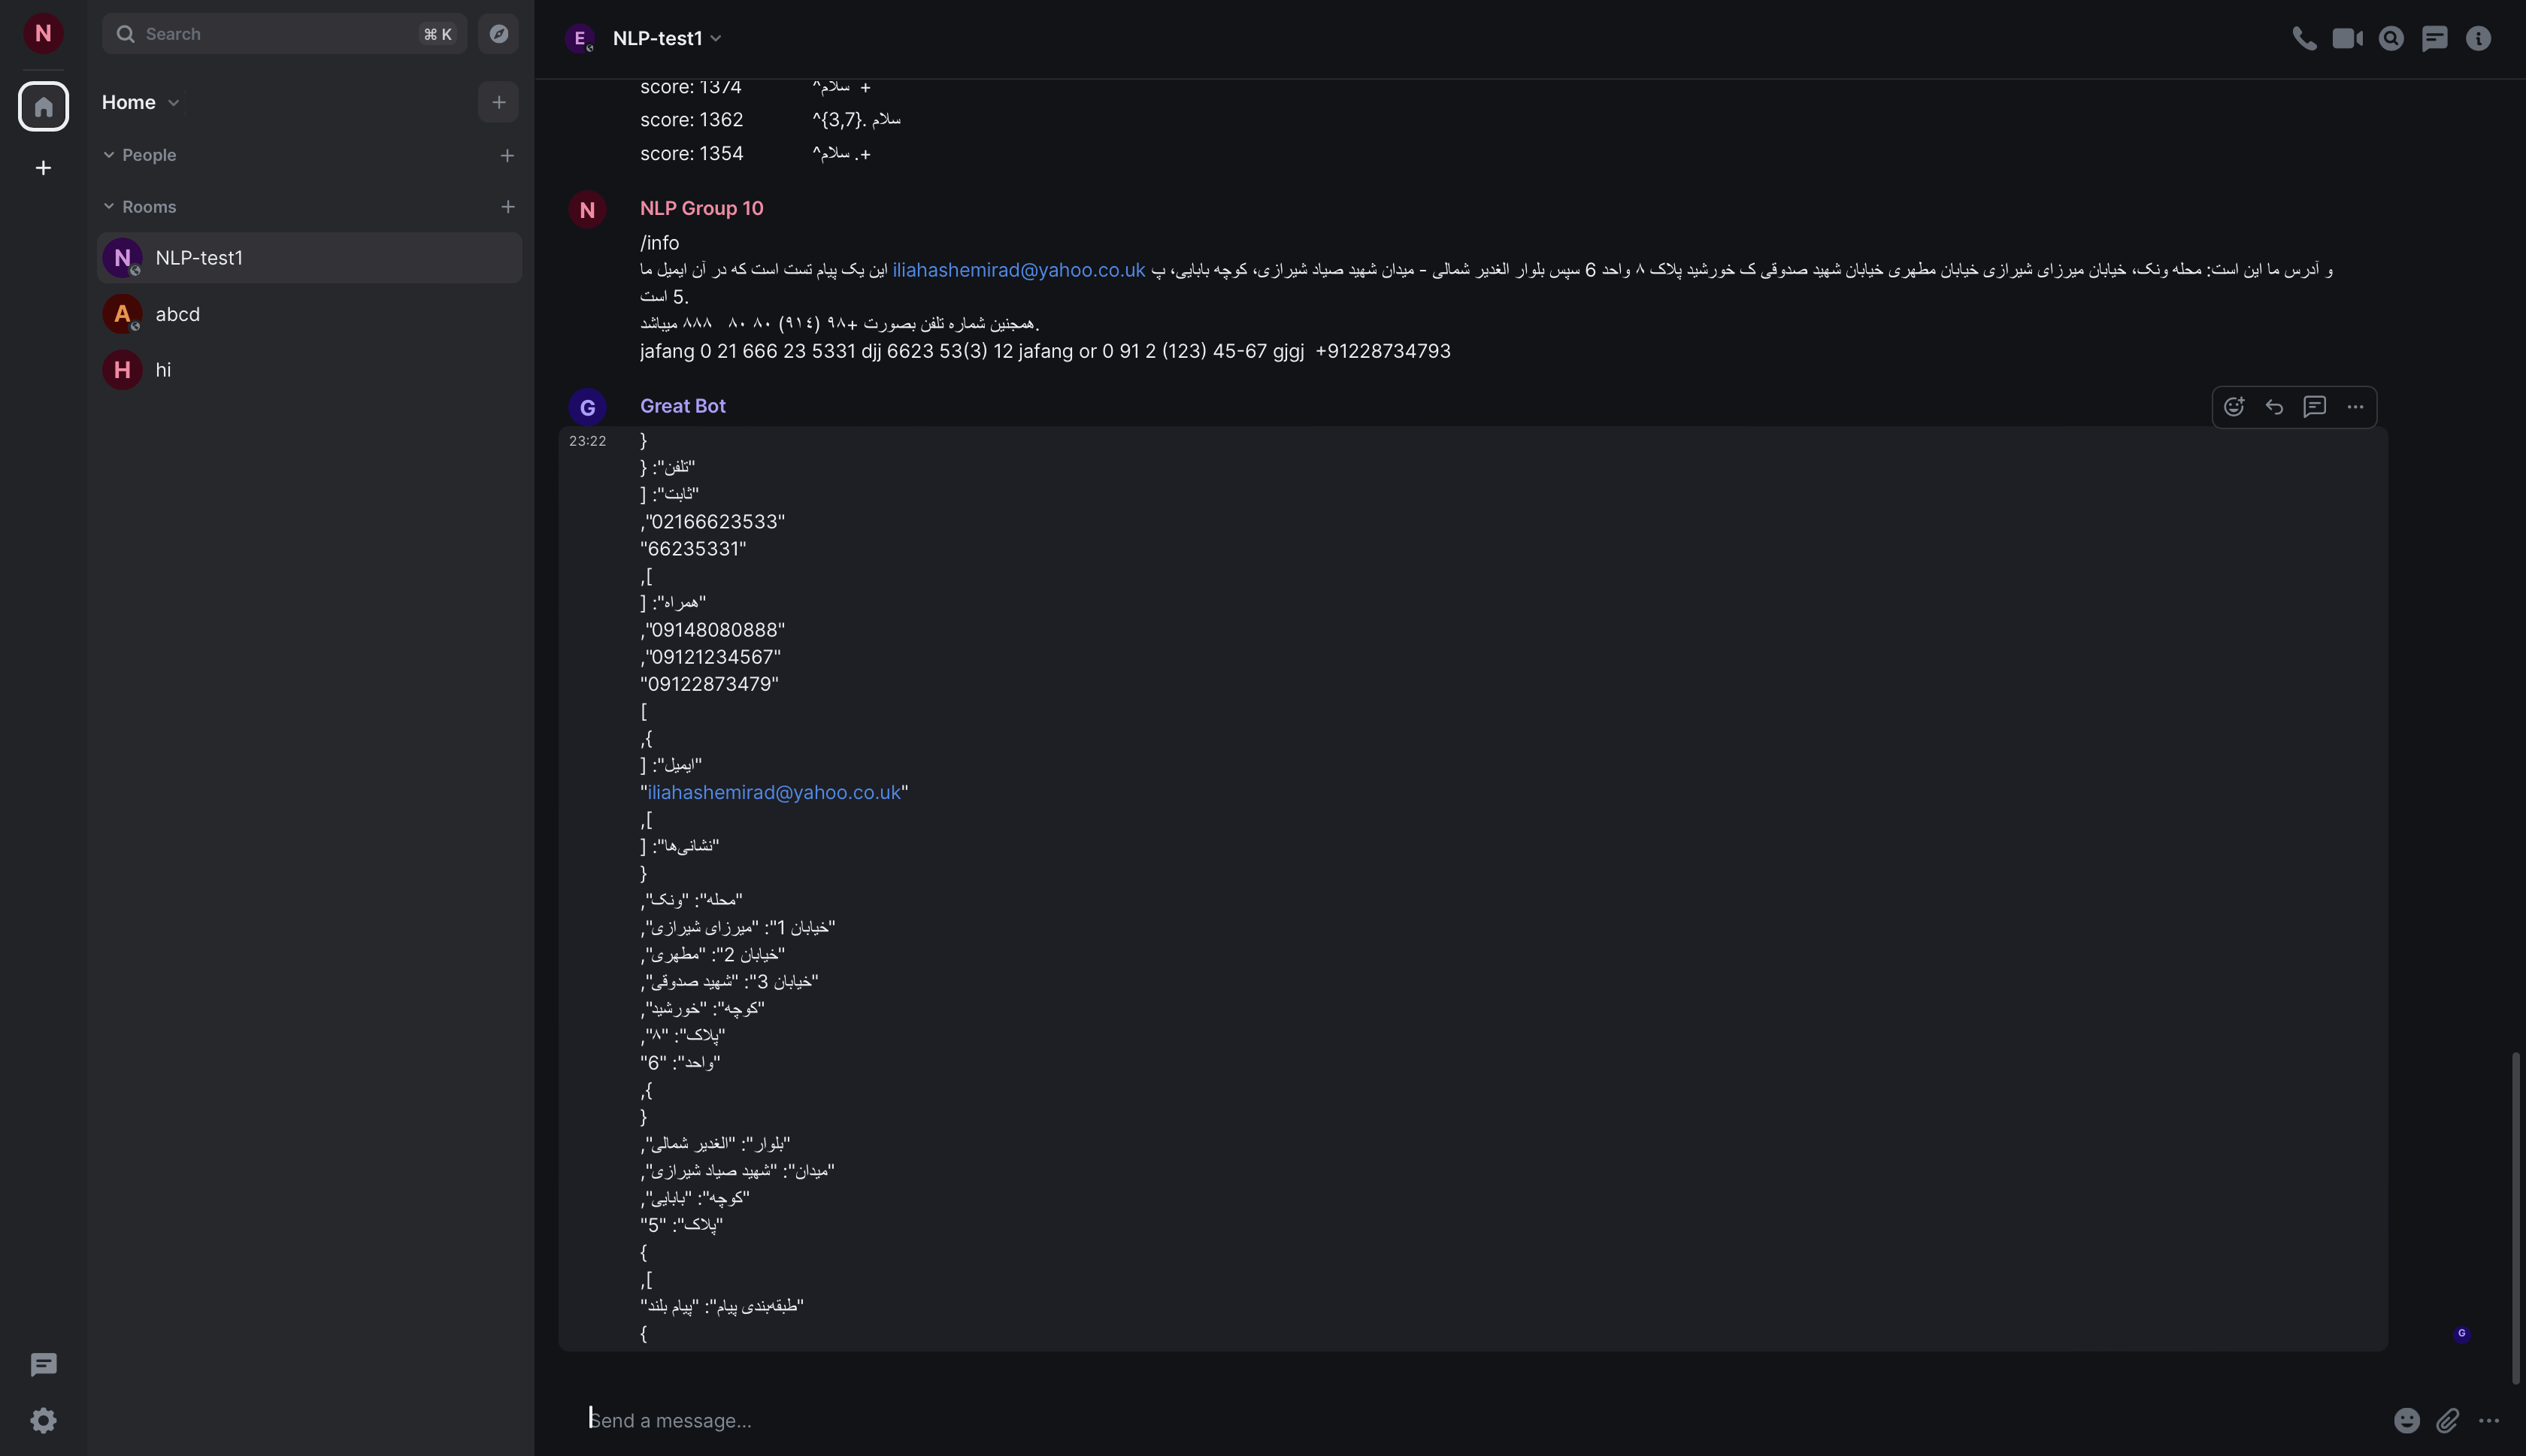
\includegraphics[scale = 0.3]{img/1.png}
\end{center}
\end{document}












